\documentclass{beamer}

% Theme
\usetheme{default}

% Packages
\usepackage{graphicx} % for including images
\usepackage{hyperref} % for hyperlinks
\usepackage{listings} % for including code

% Title
\title{Introducción a programación competitiva}
\author{Alonso Huerta}
\institute{Olimpiada Mexicana de Informática en Yucatán}
\date{\today}

% Begin document
\begin{document}

% Title slide
\begin{frame}
  \titlepage
\end{frame}

% Table of contents
\begin{frame}
  \frametitle{Tabla de Contenidos}
  \tableofcontents
\end{frame}

\section{¿Qué es la OMI?}

\begin{frame}
  \frametitle{¿Qué es la OMI?}
La Olimpiada Mexicana de Informática (OMI) es un concurso a nivel nacional para jóvenes con facilidad para resolver problemas prácticos mediante la lógica y el uso de computadoras, que busca promover el desarrollo tecnológico en México y encontrar a los mejores programadores, quienes formarán la selección mexicana para participar en las próximas Olimpiadas Internacionales de Informática (IOI).
\end{frame}

\begin{frame}
  \frametitle{Ejemplo}
	¿Cuál es el camino más rápido de inicio a fin?
	\begin{center}
		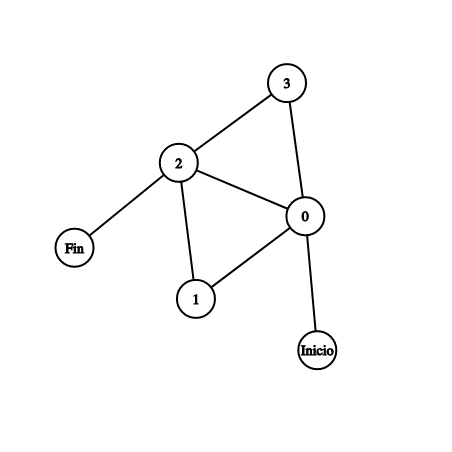
\includegraphics[width=0.6\textwidth]{img/facil.png}
	\end{center}
\end{frame}

\begin{frame}
  \frametitle{Ejemplo}
	¿Cuál es el camino más rápido de inicio a fin?
	\begin{center}
		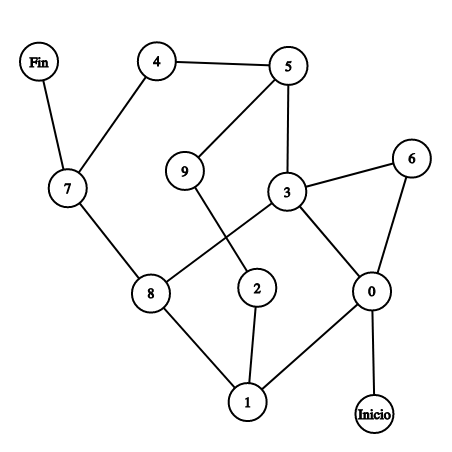
\includegraphics[width=0.6\textwidth]{img/medio.png}
	\end{center}
\end{frame}

\begin{frame}
  \frametitle{Ejemplo}
	¿Cuál es el camino más rápido de inicio a fin?
	\begin{center}
		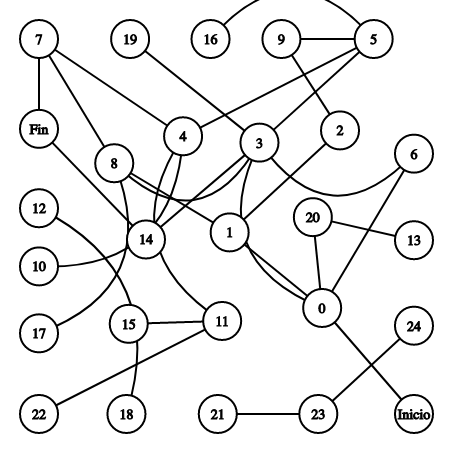
\includegraphics[width=0.6\textwidth]{img/dificil.png}
	\end{center}
\end{frame}

\begin{frame}
  \frametitle{OMM $\sim$ OMI}
	Parecidos
	\begin{itemize}
		\item Se usan matemáticas
		\item Tienes 3-4 horas cierto tiempo para hacer un examen de entre 3-5 preguntas
		\item Los problemas tienen puntos paricales y completos
	\end{itemize}
	Diferentes
	\begin{itemize}
		\item Otro tipo de matemáticas
		\item No necesitas demostrar tu solución
		\item Calificación en tiempo real
	\end{itemize}
\end{frame}

\begin{frame}
  \frametitle{OMM $\sim$ OMI}
	\begin{center}
		
\includegraphics[width=0.8\textwidth]{img/memingo.jpg}
	\end{center}
\end{frame}

\section{¿Cómo empiezo?}

\begin{frame}
  \frametitle{Aplicación: Code::Blocks}
	\begin{itemize}
		\item Reglamento: En cada examen se le proporcionará al participante: Una computadora personal, con el sistema operativo, compiladores y programas autorizados en la OMI...
		\item Compiladores autorizados: Los compiladores que se utilizan tanto en la Olimpiada Mexicana de Informática: Code::Blocks
	\end{itemize}
\end{frame}

\begin{frame}
  \frametitle{¿Y si tengo Mac?}
	\begin{center}
		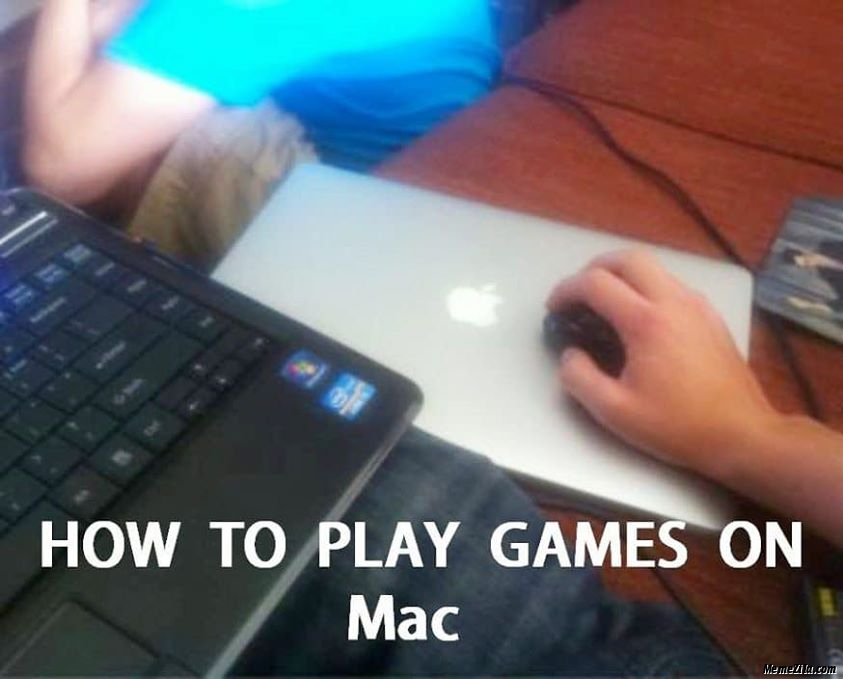
\includegraphics[width=0.8\textwidth]{img/mac.jpg}
	\end{center}
\end{frame}

\begin{frame}
  \frametitle{Plataforma de evaluación}
	\begin{center}
		
\includegraphics[width=0.8\textwidth]{img/omegaup.png}
	\end{center}
\end{frame}

\begin{frame}
  \frametitle{Obtén ayuda}
	\begin{itemize}
		\item OMIYUC  https://discord.gg/zpTbPq4yYj 
		\begin{itemize}
			\item Pregúntanos a los maestros. Material de practica.
		\end{itemize}
		\item OMI https://discord.gg/2hAp3zYQJm
		\item TPH https://discord.gg/q4KdJFP
	\end{itemize}
\end{frame}

\begin{frame}
  \frametitle{Manual de preparación}
	\begin{center}
		
\includegraphics[width=0.6\textwidth]{img/QR.jpg}
	\end{center}
\end{frame}

\section{Let's Code}

\begin{frame}
	\begin{center}
		
\includegraphics[width=0.8\textwidth]{img/letscode.jpg}
	\end{center}
\end{frame}

% End document
\end{document}
